\subsubsection{generation.mapgeneration}
    Mapgeneration bildet die Schnittstelle nach außen, für den gesammten Generierungsprozess. Hiermit lässt sich 
    die prozedurale Generierung anregen, welche dann auf die untergeordneten Generatoren verteilt wird. Ist der 
    Prozess abgeschlossen, so erhält man ein Objekte vom Typ \textit{IMapBody} zurück, welches die Strecke repräsentiert.

    \begin{figure}[htbp]
        \centering
        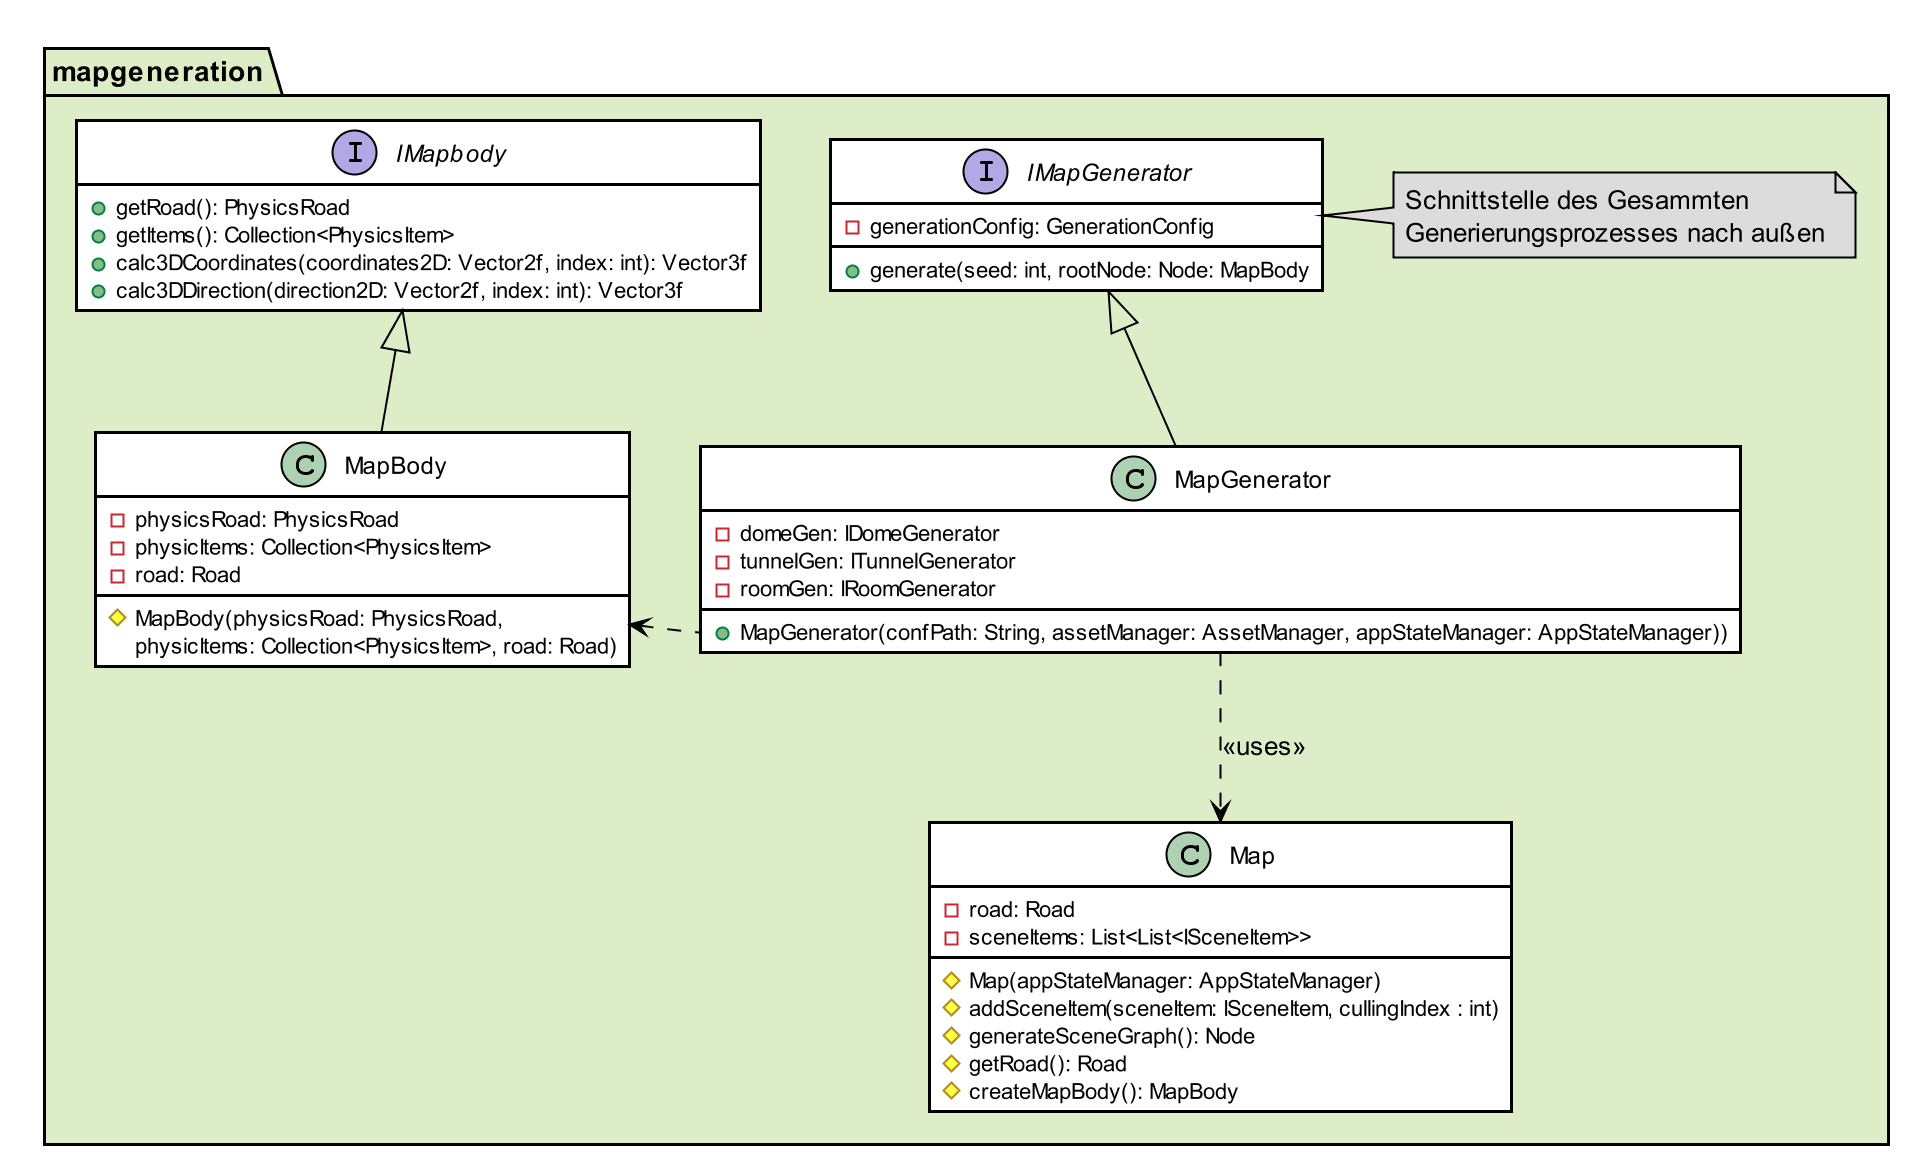
\includegraphics[width=\linewidth]{./Generierung/Bilder/mapgeneration.png}
        \caption{Klassendiagramm mapgeneration}
    \end{figure}


    \paragraph{\underline{IMapGenerator}} \mbox{}\par
            Schnittstelle, welche angesprochen werden kann um die prozedurale Generierung eine Karte, abhängig von 
            einem Seed, zu starten.\par
            
            \textbf{Methoden}					
            \begin{itemize}
                \item  \textit{+ generate(int seed, Node rootNode): MapBody}
                    \begin{leftbar}[0.9\linewidth]
                        Methode, welche die Generierung einer Karte, abhängig vom \textit{seed} einleitet
                         und dadurch einen \textit{IMapBody} zu erzeugen.\\
                        \textbf{@param seed} Zum generieren von Pseudozufallswerten.\\
                        \textbf{@param rootNode} Verwendet wie in \textit{JMonkey}, hier sollen alle Elemente der Karte 
                        angehängt werden.\\
                        \textbf{@return} Objekt einer Datenstruktur, dass die gesammte Strecke der Karte repräsentiert.
                    \end{leftbar} 
            \end{itemize}
    
    
    
        \paragraph{\underline{MapGenerator}} \mbox{}\par
            Implementiert \textit{IMapGenerator} und legt somit eine konkrete Implementierung für die Generierung fest.\par
            
            \textbf{Attribute}
            \begin{itemize}
                \item  \textit{- GenerationConfig generationConfig} 
                    \begin{leftbar}[0.9\linewidth]
                        Datenstruktur, die Parameter für die Generierung hält.
                    \end{leftbar}
                \item  \textit{- IDomeGenerator domeGen} 
                    \begin{leftbar}[0.9\linewidth]
                        Generator, der sich um die Generirung von Kuppeln kümmert.
                    \end{leftbar}
                \item  \textit{- ITunnelGenerator tunnelGen} 
                    \begin{leftbar}[0.9\linewidth]
                        Generator, der sich um die Generirung von Tunneln kümmert.
                    \end{leftbar}
                \item  \textit{- IRoomGenerator rommGen} 
                    \begin{leftbar}[0.9\linewidth]
                        Generator, der sich um die Generirung von Räumen kümmert.
                    \end{leftbar}
            \end{itemize}

            \textbf{Methoden}					
            \begin{itemize}
                \item  \textit{+ MapGenerator(String confPath, AssetManager assetManager)}
                    \begin{leftbar}[0.9\linewidth]
                        Konsrtuktor für \textit{MapGenerator}.\\
                        \textbf{@param confPath} Pfad zum JSON - Dokument, welches Parameter für die Generierung bereit hält.\\
                        \textbf{@param assetManager} Von \textit{JMonkey} vordefinierte Klasse, zum verwalten von Assets.
                    \end{leftbar}  
            \end{itemize}
    
    
    
        \paragraph{\underline{Map}} \mbox{}\par
            Datenstruktur, die die Karte während des Generierungsprozess repräsentiert. Enthält außerdem Funktionalität um einen 
            \textit{IMapBody} zu erzeugen.\par
            
            \textbf{Attribute}
            \begin{itemize}
                \item  \textit{- Road road} 
                    \begin{leftbar}[0.9\linewidth]
                        Repräsentiert die Straße, die durch die Karte verläuft.
                    \end{leftbar}
                
                \item  \textit{- List<List<ISceneItem>> sceneItems} 
                    \begin{leftbar}[0.9\linewidth]
                        Liste an \textit{sceneItems}, welche jeweils einen \textit{cullingIndex} besitzen.
                    \end{leftbar}
            \end{itemize}

            \pagebreak
            \textbf{Methoden}					
            \begin{itemize}
                \item  \textit{\# Map(appStateManager: AppStateManager)}
                    \begin{leftbar}[0.9\linewidth]
                        Konsrtuktor für \textit{Map}.\\
                        \textbf{@param appStateManager} Von \textit{JMonkey}übernommen, zum verwalten der \textit{Appstates}.
                    \end{leftbar}

                \item  \textit{\# addSceneItem(ISceneItem sceneItem, int cullingIndex)}
                    \begin{leftbar}[0.9\linewidth]
                        Fügt ein \textit{ISceneItem} zur Karte hinzu und erweitert diese so.\\
                        \textbf{@param sceneItem} Datenstruktur die einen Abschnitt der Karte, wie beispielsweise eine Kuppel, 
                        repräsentiert.
                        \textbf{@param cullingIndex} Nummerierung der Teilabschnitte einer Karte.
                    \end{leftbar}    
        
                \item  \textit{\# generateSceneGraph(): Node}
                    \begin{leftbar}[0.9\linewidth]
                        Gibt den SceneGraph, wie in \textit{JMonkex} verwendet, für die Karte zurück.\\
                        \textbf{@return} Verwendet wie in \textit{JMonkey}, wird übergeben um die Karte in einer Szene darzustellen.
                    \end{leftbar}    
            
                \item  \textit{\# getRoad(): Road}
                    \begin{leftbar}[0.9\linewidth]
                        \textbf{@return} Datenstruktur, die den Streckenverlauf der Karte beschreibt.
                    \end{leftbar}    
                
                \item  \textit{\# createMapBody(): MapBody}
                    \begin{leftbar}[0.9\linewidth]
                        \textbf{@return} Objekt einer Datenstruktur, dass die gesammte Strecke der Karte repräsentiert.
                    \end{leftbar}    
            \end{itemize}
    
    
    
         \paragraph{\underline{IMapBody}} \mbox{}\par
         Datenstruktur, die einen Streckenverlauf einer Karte repräsentiert. Hieru werden auch alle Objekte, die auf dieser 
         platziert sind gehalten.\par
            
            \textbf{Methoden}					
            \begin{itemize}
                \item  \textit{+ getRoad(): PhysicsRoad}
                \begin{leftbar}[0.9\linewidth]
                        \textbf{@return} Datenstruktur einer Strecke, die durch das andere Team definiert wird.
                    \end{leftbar}
                    
                    \item  \textit{+ getItems(): Collection<PhysicsItem>}
                    \begin{leftbar}[0.9\linewidth]
                        \textbf{@return} Datenstruktur, die Objekte auf der Strecke darstellt, definiert durch das andere Team.
                    \end{leftbar}    
                    
                    \item  \textit{+ calc3DCoordinates(Vector2f coordinates2D, int index): Vector3f}
                    \begin{leftbar}[0.9\linewidth]
                        Berechnet die 3D - Weltkoordinaten aus dem 2D - System des anderen Teams.\\
                        \textbf{@param coordinates2D} 2D - Koordinate aus dem System des anderen Teams.\\
                        \textbf{@param index} Indiziert einen \textit{RaodCursor} im Streckenverlauf.\\
                        \textbf{@return} 3D - Koordinate des Darstellungstyps \textit{Map} der Karte.
                    \end{leftbar}
                    
                    \item  \textit{+ calc3DDirection(Vector2f direction2D, int index): Vector3f}
                    \begin{leftbar}[0.9\linewidth]
                        Berechnet eine 3D - Vektor, der eine Richtung angibt, aus dem 2D - System des anderen Teams.\\
                        \textbf{@param direction2D} 2D - Vektor aus dem System des anderen Teams.\\
                        \textbf{@param index} Indiziert einen \textit{RaodCursor} im Streckenverlauf.\\
                        \textbf{@return} 3D - Vektor für eine Richtung im Darstellungstyp \textit{Map} der Karte.
                    \end{leftbar}    
                \end{itemize}
                
                
                
            \paragraph{\underline{MapBody}} \mbox{}\par
                Implementiert \textit{IMapBody} und implementiert somit die konkreten Brechnungen für das System des anderen Teams.
                    
                \textbf{Attribute}
                \begin{itemize}
                    \item  \textit{- PhysicsRoad physicsRoad} 
                        \begin{leftbar}[0.9\linewidth]
                            Datenstruktur einer Strecke, die durch das andere Team definiert wird.
                        \end{leftbar}
                
                    \item  \textit{- Collection<PhysicsItem> physicItems} 
                        \begin{leftbar}[0.9\linewidth]
                            Datenstruktur, die Objekte auf der Strecke darstellt, definiert durch das andere Team.
                        \end{leftbar}
                    
                    \item  \textit{- Road road} 
                        \begin{leftbar}[0.9\linewidth]
                            Datenstruktur den Streckenverlauf der Karte repräsentiert.
                        \end{leftbar}
                \end{itemize}
    
                \textbf{Methoden}					
                \begin{itemize}
                    \item  \textit{\# MapBody(PhysicsRoad physicsRoad, Collection<PhysicsItem> physicItems, Road road)}
                        \begin{leftbar}[0.9\linewidth]
                            Konsrtuktor für \textit{MapBody}.\\
                            \textbf{@param physicsRoad} Datenstruktur einer Strecke, die durch das andere Team definiert wird.\\
                            \textbf{@param physicItems} Datenstruktur, die Objekte auf der Strecke darstellt, definiert durch das andere Team.\\
                            \textbf{@param road} Datenstruktur den Streckenverlauf der Karte repräsentiert.\\
                        \end{leftbar}  
                \end{itemize}
